\documentclass{article}
\usepackage[utf8]{inputenc}

\usepackage{hyperref}
\usepackage{longtable}
\usepackage{listings}
\usepackage{tabularx}
\usepackage{verbatim}
\usepackage{graphicx}

%Gebaseerd op IEEE Std 1058-1998

\begin{document}

\begin{titlepage}
\title{Software Project Management Plan \\ WiseLib}
\date{14 December 2014}
\author{Wout Van Riel \\ Yannick Verschueren \\ Sam Vervaeck \\ Arno Moonens \\ Mathieu Reymond \\ se2-1415}
\end{titlepage}

\maketitle

\newpage
\tableofcontents

\newpage

\begin{table}[h]
\centering
\begin{tabular}{c|c|c}
Versie & Auteur & Commentaar \\
\hline
 version 0.1 & Wout Van Riel & Eerste versie\\
 version 0.2 & Wout Van Riel & Eerste versie verbetert\\
 version 1.0 & Wout Van Riel & SPMP aangepast met behulp van de standaard \\
 version 1.1 & Wout Van Riel & SPMP up-to-date gebracht \\
 version 1.2 & Wout Van Riel & Nakijken op spellingsfouten

\end{tabular}

\caption{Revision Chart}
\label{tab:revchart}
\end{table}

\section{Introductie}



\subsection{Projectbeschrijving}
\subsubsection{Doel en objectieven}

Dit project heeft als doel een webtoepassing te creëren waar men publicaties op kan plaatsen en beheren.  Het project is onderdeel van het vak Software Engineering dat gegeven wordt door Ragnhild Van Der Straeten \cite{rvdstrae} aan de Vrije Universiteit Brussel. De vereisten die gegeven zijn voor dit project, worden beschreven in het SRS.

\subsubsection{Veronderstellingen en beperkingen}
\paragraph{Veronderstellingen}
We gaan er van uit dat de toepassing op verschillende toestellen gaat werken, zodat mensen overal aan publicaties kunnen geraken. Na deze iteratie werkt de toepassing enkel nog maar op een computer maar in latere iteraties zal hier aan worden gewerkt.

\paragraph{Beperkingen}
\begin{itemize}
\item Het systeem moet werken onder Wilma \cite{Wilma} en een up-to-date browser. %LINK wilma
\item GitHub \cite{GitHub} moet gebruikt worden als repository.
\item Enkel JavaScript, HTML5, CSS en bijbehorende open-source frameworks en bibliotheken mogen worden gebruikt als programmeertaal of technologie.
\item Enkel vrije software mag gebruikt worden, zowel voor het eindproduct als voor hulpmiddelen.
\item Het systeem moet eenvoudig kunnen ge\"installeerd worden, op een standaard manier.
\item De grafische gebruikersinterface moet aantrekkelijk en eenvoudig zijn.
\end{itemize}

\subsubsection{Project Deliverables}

In onderstaande tabellen staan de data wanneer de documenten \ref{tab:doc} en de code \ref{tab:code} worden afgeleverd en wanneer presentaties \ref{tab:pres} over het project worden gegeven. 

\begin{table}[h]
\begin{minipage}[b]{0.45\linewidth}
\begin{tabularx}{1.9\textwidth}{c|c}
\hline
\textbf{Datum} & \textbf{Documenten}\\
 \hline
 Woensdag 05/11/2014 & inleveren SPMP \\
 Woensdag 19/11/2014 & eerste versie documenten \\
 Maandag 15/12/2014 & Einde iteratie 1: opleveren documenten \\
 \hline \hline
 Dinsdag 03/03/2015 & Einde iteratie 2: opleveren documenten \\
 Maandag 20/04/2015 & Einde iteratie 3: opleveren documenten \\
 Vrijdag 15/05/2015 & Einde iteratie 4: finale oplevering
\end{tabularx}
\caption{Documenten}
\label{tab:doc}
\end{minipage}

\vspace{0.5cm}

\begin{minipage}[b]{0.45\linewidth}
\begin{tabularx}{1.9\textwidth}{c|c}
\hline
\textbf{Datum} & \textbf{Code}\\
 \hline
 Maandag 15/12/2014 & Einde iteratie 1: opleveren code \\
 \hline \hline
 Dinsdag 03/03/2015 & Einde iteratie 2: opleveren code \\
 Maandag 20/04/2015 & Einde iteratie 3: opleveren code \\
 Vrijdag 15/05/2015 & Einde iteratie 4: finale oplevering
\end{tabularx}
\caption{Code}
\label{tab:code}
\end{minipage}
\vspace{0.5cm}

\begin{minipage}[b]{0.45\linewidth}
\begin{tabularx}{1.9\textwidth}{c|c}
\hline
\textbf{Datum} & \textbf{Presentaties}\\
 \hline
 Vrijdag 19/12/2014 & presentatie 1 \\
 \hline \hline
Woensdag 11/03/2015 & presentatie 2\\
Woensdag 22/04/2015 & presentatie 3\\
Woensdag 20/05/2015 & finale presentatie\\
\end{tabularx}
\caption{Presentaties}
\label{tab:pres}
\end{minipage}
\end{table}
\newpage

De documenten die telkens afgeleverd worden, zijn de volgende:

\begin{itemize}
\item Software Project Management Plan (SPMP)
\item Software Test Plan (STD)
\item Software Requirements Specification (SRS)
\item Software Design Document (SDD)
\item Minutes van alle vergaderingen
\end{itemize}

\newpage  
\subsubsection{Planning}
\begin{figure}[h]
\centering
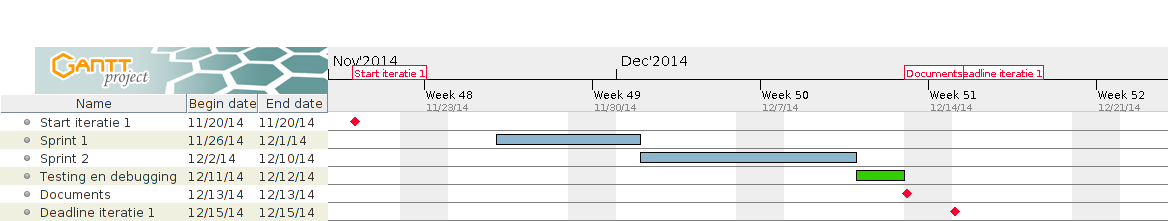
\includegraphics[width=1.2\linewidth]{./document.png}
\caption{Planning iteratie 1}
\label{fig:planning}
\end{figure}

  

\subsection{Evolutie van het SPMP}
De eerste versie van het SPMP wordt ingeleverd op 5 november 2014. Daarna zal bij elke iteratie een geüpdate versie van het SPMP worden meegegeven. De geschiedenis van het SPMP is gegeven in tabel \ref{tab:revchart}. De verantwoordelijkheid van dit document ligt bij de project manager. Dit SPMP volgt voornamelijk de standaard IEEE 1058-1998 \cite{ieeestd}.

\section{Referentiemateriaal}

\begin{thebibliography}{9}
\bibitem{ieeestd} \emph{IEEE Std 1058-1998}  
\bibitem{Website} \emph{Team Website} \url{http://wilma.vub.ac.be/~se2_1415/} \\
\bibitem{Wilma} \emph{Wilma} \url{http://wilma.vub.ac.be}\\
\bibitem{GitHub} \emph{GitHub Repository} \url{https://github.com/wiselib} \\
\bibitem{Teamwork} \emph{Teamwork} \url{https://wiselib.teamwork.com} \\
\bibitem{Slack} \emph{Slack} \url{https://wiselib.slack.com} \\
\bibitem{Sharelatex} \emph{ShareLa-eX} \url{https://www.sharelatex.com} \\

\bibitem{rvdstrae} \emph{Ragnhild Van Der Straeten} \href{mailto:rvdstrea@vub.ac.be}{rvdstrea@vub.ac.be} \\
\bibitem{jnicolay} \emph{Jens Nicolay} \href{mailto:jnicolay@vub.ac.be}{jnicolay@vub.ac.be} 
\bibitem{dvdeun} \emph{Dirk van Deun} \href{mailto:dirk@dinf.vub.ac.be}{dirk@dinf.vub.ac.be}
\end{thebibliography}

\section{Defenities en Acroniemen}

\begin{table}[h]
\centering
\begin{tabular}{c|c}
\textbf{Acroniem} & \textbf{Betekenis} \\
\hline
SPMP & Software Project Management Plan  \\
SRS & Software Requirements Specification \\
STP & Software Test Plan \\
SDD & Software Design Document \\
SQAP & Software Quality Assurance Plan \\
SCMP & Software Configuration Management Plan \\
VUB & Vrije Universiteit Brussel
\end{tabular}
\caption{Ancroniemen}
\label{tab:my_label}
\end{table}

\section{Project organisatie}

\subsection{Externe interfaces}
Het project is opgedragen door de VUB in het kader van de lessen "Software Engineering". De cliënten zijn Ragnhild Van Der Straeten \cite{rvdstrae} en assistent Jens Nicolay \cite{jnicolay}. De applicatie zal initieel op Wilma \cite{Wilma} staan, een multifunctionele Linux-server die wordt onderhouden door Dirk van Deun \cite{dvdeun}. \\

\subsection{Interne structuur}

\begin{figure}[h]
\centering
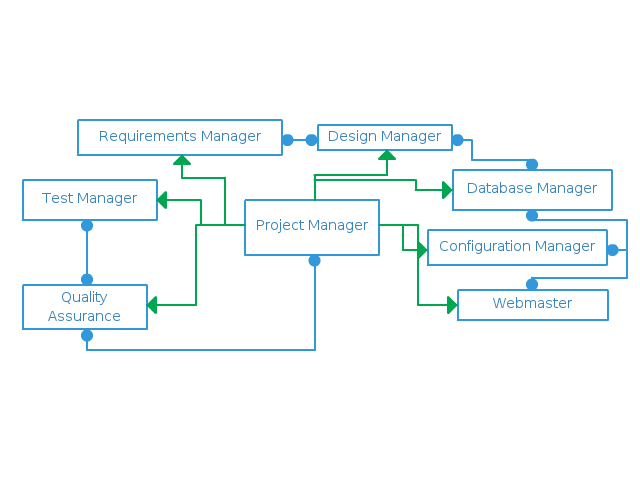
\includegraphics[width=\linewidth]{./Wiselib_intOrg.png}
\caption{Interne organisatie}
\label{fig:intorg}
\end{figure}

De groene pijlen duiden aan wie toezicht houdt over wie.\newline 
De blauwe pijlen duiden aan tussen wie er veel gecomuniceerd wordt.

\subsection{Rollen en verantwoordelijkheden}
De teamleden vullen verschillende rollen in.
De rollen en hun functies zijn: 

\begin{itemize}
\item Project Manager
\begin{itemize}
\item Leidt het team
\item Contactpersoon van het team
\item Bemiddelaar tijdens meningsverschillen
\item Verantwoordelijk voor de vergaderingen
\item Maakt SPMP en onderhoudt het
\end{itemize}

\item Configuration Manager
\begin{itemize}
\item Beheert de tools en libraries die gebruikt worden
\item Beheert GitHub
\item Maakt het SCMP en onderhoudt het
\end{itemize}

\item Database Manager
\begin{itemize}
\item Beheert de database
\item Maakt en onderhoudt het SDD samen met de Design Manager
\end{itemize}

\item Design Manager
\begin{itemize}
\item Maakt en onderhoudt het SDD 
\item Beslist en beheert het design van de toepassing en de database
\item Communiceert met de cliënt over het design
\end{itemize}

\item Test Manager
\begin{itemize}
\item Zorgt dat het programma aan voldoende testen wordt onderworpen
\item Documenteert en rapporteert de resultaten van de testen
\item Maakt een test database aan
\item Maakt en onderhoudt het STD
\end{itemize}

\item Quality Assurance
 \begin{itemize}
 \item Zorgt voor de kwaliteit van de code
 \item Is verantwoordelijk voor de kwaliteit van de applicatie
 \item Zorgt ervoor dat aan alle nodige requirements voldaan zijn
 \item Maakt en onderhoudt het SQAP
 \end{itemize}
 
\item Requirements Manager
\begin{itemize}
\item Maakt en onderhoudt het SRS
\item Beslist de prioriteiten van de requirements
\item Communiceert met de cliënt over de requirements
\end{itemize}

\item Webmaster 
\begin{itemize}
\item Maakt en onderhoudt de website
\end{itemize}
\end{itemize}
 \newpage



\section {Leidinggevende werkwijze plan} 

\subsection{Start-up plan}
\subsubsection{Personeelsbezetting}
De groep die aan dit project werkt, is samengesteld door professor Raghnild Van Der Straeten \cite{rvdstrae} en haar assistent Jens Nicolay\cite{jnicolay}. In totaal bestaat de groep uit vijf personen en er is geen mogelijkheid om nieuwe werkkrachten in te huren. Er kan altijd een persoon wegvallen uit de groep. Dit kan door persoonlijke redenen of omdat hij niet in de groep kan functioneren. Als iemand uit de groep wil gaan, zal dit intern en met de professor besproken worden.
In de onderstaande tabel staan de functies en de personen die verantwoordelijk en back-up zijn voor deze functies.

\begin{table}[h]
\centering
\begin{tabular}{c|c|c}
\textbf{Rol} & \textbf{Verantwoordelijke} & \textbf{Back-up}  \\
\hline
 Project Manager & Wout Van Riel & Mathieu Reymond \\
 Design Manager & Mathieu Reymond & Yannick Verschueren \\
 Requirements Manager & Mathieu Reymond & Yannick Verschueren \\
 Test Manager & Yannick Verschueren & Arno Moonens \\
 Quality Assurance & Yannick Verschueren & Arno Moonens \\
 Database Manager & Arno Moonens & Sam Vervaeck \\
 Config Manager & Sam Vervaeck & Wout Van Riel \\
 Webmaster & Sam Vervaeck & Wout Van Riel
\end{tabular}
\caption{Rolverdeling}
\label{tab:rolverdeling}
\end{table}

\subsubsection{Plan om middelen te werven}
Er wordt enkel gebruik gemaakt van vrije software. Dit project heeft geen budget om mee te werken en zal dus dienst doen op vrije software. Het is ook een vereiste die is meegegeven met het project. 

\subsubsection{Trainingsplan}
In onderstaande tabel staan de onderdelen waar het personeel in getraind moeten worden. Naast elk onderdeel staat de wijze hoe het personeel opgeleid zal worden.

\begin{table}[h]
\begin{tabular}{l|l}
LaTeX      & Tutorials en documentatie \\
Javascript & Tutorials en documentatie  \\
HTML       & Tutorials en documentatie  \\
CSS        & Tutorials en documentatie 
\end{tabular}
\caption{Trainingstabel}
\label{tab:training}
\end{table}

\subsection{Werkplan}
\subsubsection{Werk activiteiten}
\begin{table}[h]
\begin{tabular}{l|l|l|c|c|c}
\textbf{Activiteit} & \textbf{Verantwoordelijke} & \textbf{Duur} & \textbf{Document} & \textbf{\begin{tabular}[c]{@{}c@{}}Voorafgaand\\ Document\end{tabular}} & \textbf{\begin{tabular}[c]{@{}c@{}}Opvolgend\\ Document\end{tabular}} \\ \hline
Beheer              & Project Manager            & 30u           & SPMP              &                                                                         &                                                                       \\
Kwaliteit           & Quality Assurance          & 25u           & SQAP              &                                                                         &                                                                       \\
Testen              & Test Manager               & 25u           & STD               &                                                                         &                                                                       \\
Design              & Design Manager             & 25u           & SDD               & SRS                                                                     &                                                                       \\
Vereisten           & Requirements Manager       & 25u           & SRS               &                                                                         & SDD                                                                   \\
Configuratie        & Configuration Manager      & 25u           & SCMP              &                                                                         &                                                                      
\end{tabular}
\caption{Werk activiteiten}
\label{tab:werkAct}
\end{table}

\subsubsection{Werkplanning}

De werkplanning is te zien in figuur ~\ref{fig:planning}.

\subsection{Controle plan}
\subsubsection{Requirements controle}
Om een overzicht te houden van alle requirements zal er op de site \cite{Website} een requirements dashboard worden opgezet. Deze tabel zal de requirements bijhouden en hun prioriteit. Als een requirement is afgewerkt, wordt de requirement doorstreept in de tabel. Mogelijke aanpassingen van de requirements worden tussen de requirements manager en de cliënt besproken. Als er een requirement moet veranderen, dan moet de requirements manager dit als punt op de agenda zetten voor de volgende vergadering en past hij het SRS aan.

\subsubsection{Planning controle}

Er zijn algemene milestones en deadlines die tijdens de vergaderingen worden afgesproken. Iedereen is verantwoordelijk voor zijn eigen deadlines. Op elke vergadering vraagt de project manager aan iedereen de stand van zaken. Als er iemand zijn deadline niet kan halen, dan zal er besproken worden of er iemand anders mee kan helpen of dat de deadline kan opgeschoven worden. Mist iemand zijn deadline zonder geldige reden, dan zal de project manager die persoon daar over aanspreken en zal hij het vermelden op de volgende vergadering. De planning wordt met Teamwork \cite{Teamwork} beheerd. 

\subsubsection{Rapportering} 
\paragraph{Documenten en code} 
Op het einde van elke iteratie worden documenten, source code en (eventueel) andere artefacten opgeleverd.
Afspraken in verband met deze opleveringen: 

\begin{itemize}
\item Alle documenten en source code (inclusief unit tests) worden per mail afgeleverd als een
enkele zipfile, met als naam se2-iterM, waarbij M het nummer van de iteratie is (voor
eerste versie van documenten geldt M = 0). De aanlevering gebeurt ten laatste voor 9u00 ’s
ochtends op de dag van de deadline.
\item Alle documenten en source code worden worden overeenkomstig getagd/gebranchd (se2-iterM)
in de repository.
\item Andere artefacten (zoals executables) worden apart aangeleverd (direct, of via een link, in de
opleveringsmail) en vermelden duidelijk de overeenkomstige iteratie in de bestandsnaam.
\item De mail van de oplevering bevat een bondig overzicht (lijstje) van wat er precies opgeleverd
wordt.
\end{itemize}

\paragraph{Presentatie}
Een presentatie duurt een half uur per groep en wordt ingevuld door een aantal sprekers, met 2 sprekers
per groep. Alle groepsleden moeten minimum een keer presenteren. De volgende zaken worden
besproken of gedemonstreerd:

\begin{itemize}
\item een demo van de toegevoegde functionaliteit ten opzichte van de vorige iteratie: gebruik requirements
dashboard, en toon een testrapport (aantal tests, aantal succesvol)
\item analyse van de ontmoette obstakels en de genomen beslissingen
\item bespreking van de functionaliteiten die aan bod zullen komen in de volgende iteratie
\item bespreking van eventuele obstakels, risico’s, etc. in de volgende iteratie
\item overzicht van de architectuur en design van de applicatie
\item bespreking van de statistieken zoals de tijd per taak en per persoon en van de eventuele vertragingen
(plus oplossingen om deze zo klein mogelijk te houden en te vermijden in de toekomst)
\end{itemize}

\subsection{Risico Management Plan}

\paragraph{Eén van de teamleden is ziek of verlaat het team}
\begin{itemize}
\item Kans: 4
\item Impact: 6
\item Prioriteit: 7
\item Oplossing: De Back-up neemt de positie van het teamlid over
\item Verantwoordelijkheid: Project Manager
\end{itemize}

\paragraph{Slechte communicatie binnen de groep}
\begin{itemize}
\item Kans: 6
\item Impact: 5
\item Prioriteit: 7
\item Oplossing: Er worden algemene afspraken gemaakt over de communicatie
\item Verantwoordelijkheid: Project Manager
\end{itemize}

\paragraph{Een deadline wordt gemist}
\begin{itemize}
\item Kans: 2
\item Impact: 9
\item Prioriteit: 7
\item Oplossing: Alle voortgang wordt op github geplaatst, elk teamlid geeft elke week zijn status op de vergadering
\item Verantwoordelijkheid: Project Manager
\end{itemize}

\paragraph{Miscommunicatie tussen de cliënt en het team}
\begin{itemize}
\item Kans: 2
\item Impact: 7
\item Prioriteit: 7
\item Oplossing: De requirements manager houdt contact met de cliënt en bespreekt onduidelijkheden met de cliënt
\item Verantwoordelijkheid: Requirements Manager
\end{itemize}

\paragraph{Plotselinge verandering in de requirements}
\begin{itemize}
\item Kans: 2
\item Impact: 5
\item Prioriteit: 5
\item Oplossing: Proberen de requirement in de bestaande code toe te voegen
\item Verantwoordelijkheid: Requirements Manager
\end{itemize}

\paragraph{Server is tijdelijk offline}
\begin{itemize}
\item Kans: 1
\item Impact: 8
\item Prioriteit: 8
\item Oplossing: Een mirror server opzetten
\item Verantwoordelijkheid: Configuration Manager
\end{itemize}

\paragraph{Onenigheid tussen de teamleden}
\begin{itemize}
\item Kans: 4
\item Impact: 6
\item Prioriteit: 8
\item Oplossing: Bemiddelen tussen de verschillende leden 
\item Verantwoordelijkheid: Project Manager
\end{itemize}

\paragraph{Database model staat de functies van het systeem niet toe}
\begin{itemize}
\item Kans: 4
\item Impact: 7
\item Prioriteit: 8
\item Oplossing: Het database model veranderen
\item Verantwoordelijkheid: Database Manager
\end{itemize}

\paragraph{Merge-conflicten in de master branch in Git}
\begin{itemize}
\item Kans: 9
\item Impact: 3
\item Prioriteit: 7
\item Oplossing: Er wordt een verantwoordelijke aangesteld die de pull requests moet goedkeuren
\item Verantwoordelijkheid: Quality Assurance
\end{itemize}


\section{Technisch proces plan}

\subsection{Proces model}

Er zal gebruik gemaakt worden van een iteratieve ontwikkeling. Dit model is gekozen vanwege de agenda waar we in verschillende iteraties code moeten afleveren. Het is ook gekozen omdat het makkelijker is om requirements per iteratie te verdelen. Zo wordt beslist aan het begin van elke iteratie welke requirements uitgewerkt zullen worden en zal het einde van de iteratie als deadline dienen voor de documenten en code.

\subsection{Methodes, Tools en Technieken}

In dit project worden enkel JavaScript, HTML5 en CSS  gebruikt. Marco-talen, zoals onder meer SASS en CoffeeScript, zullen niet aanwezig zijn in dit project. Er wordt wel gebruik gemaakt van open-source softwarebibliotheken en software-frameworks. De tools die gebruikt worden, zijn terug te vinden in het Configuration Management Plan \ref{SCMP} in tabel \ref{tab:tools}.

Alle documentatie van het project worden op de GitHub \cite{GitHub} van WiseLib geplaatst.

\subsection{Software Documentatie}

Bij elke iteratie moeten er een aantal documenten mee doorgestuurd worden. \newline
De documenten zijn de volgende:

\begin{itemize}
\item Software Project Management Plan (SPMP)
\begin{itemize}
\item Software Quality Assurance Plan (SQAP)
\item Software Configuration Management Plan (SCMP)
\end{itemize}

\item Software Test Plan (STP)
\item Software Requirements Specification (SRS)
\item Software Design Document (SDD)
\item Minutes van alle vergaderingen 
\item Code documentatie 
\end{itemize}

%\subsubsection{Documentatie van Broncode}
%komt in QA



\section{Software Quality Assurance Plan}
\label{sec:SQAP}
\subsection{Doel}

Dit document behandeld de processen en methodes die gebruikt worden in de quality assurance van het project "WiseLib". Dit document volgt de IEEE standaarden voor Quality Assurance Plannen.
\footnote{\url{http://users.csc.calpoly.edu/~jdalbey/205/Resources/IEEE7301989.pdf}}


\subsection{Referentiedocumenten}

\begin{description}
\item [SCMP] Software Configuration Mangment Plan
\end{description}

\subsection{Management}

\subsubsection{Organisatie}

De Quality Assurance wordt beheerd door Yannick Verschueren en Arno Moonens. Hierbij speelt Yannick de hoofdrol en zal Arno slechts invallen in geval van nood. De Quality Assurance Manager heeft als verantwoordelijkheid dat de gevraagde functionaliteiten van het project correct werken, en dat de geproduceerde code geen bugs meer bevat. Aangezien software ontwikkeling verdeeld wordt over het gehele team zal er dus grote afhankelijkheid zijn tussen de QA manager en de verige teamleden.

\subsubsection{Taken}

Hoewel het Quality Assurance proces gedurende het hele project loopt, zal er na de voltooiing van een functionaliteit een periode verhoogde activiteit volgen. Tijdens deze periode wordt er nagegaan of de functionaliteit op een correcte manier functioneert.
Tussen deze verschillende periode zal er uiteraard ook gewerkt aan bugs en algemeene correctheid van de code.

\subsubsection{Verantwoordelijkheden}

Aangezien het QA team uit één persoon bestaat, is de manager verantwoordelijk voor alle taken die kwaliteit verzekeren.

\begin{comment}
\subsection{Documentatie}

Niet van toepassing

\end{comment}

\subsection{Standaarden, gebruiken, conventies en metrieken}

\subsubsection {Standaarden}

\paragraph {Documentstandaarden} ~\\
De documenten gebruiken de IEEE standaarden  \footnote{\url{http://www.ieee.org/publications_standards/publications_standards_index.html}}
\begin{comment}

\paragraph{Codering standaarden}

In ontwikkeling.

\paragraph{Commentaar standaarden}

In ontwikkeling.

\end{comment}

\subsubsection{Gebruiken}

Naast het testen van de applicatie door algemeen gebruik, zal het testing framework (zie 9) gebruikt worden om correctheid van functionaliteiten te garanderen doorheen de verschillende iteraties van de applicatie. 

\subsection{Audits}

Aangezien het hele team aan de implementering van het systeem is elke vergadering waarin geschreven code wordt besproken een zowel functionele, fysieke als in-process audit.

\begin{comment}

\subsection{Test}
Niet van toepassing (SVVP (Software Verification an Validation Plan) niet vereist)

\end{comment}

\subsection{Probleem rappotrering}
Het rapporteren van problemen in zowel software als software ontwikkelings processen worden op verschillende manieren gerapporteerd.
\begin{description}
\item[Slack] het gebruikte communicatie platform bevat een "bugs" kanaal waarin problemen en bugs worden gepost.
\item[GitHub] heeft een ingebouwde issue-tracker.
\item[Trello] wordt gebruikt om grotere problemen te melden die de voortgang van de implementatie zouden kunnen hinderen.

\end{description}

\subsection{Tools, technieken en methodologieën}

Het QA proces gebruikt Mocha \footnote{\href{https://github.com/mochajs}{Mocha Homepage}} als testing-framework. Dit framework zal in combinatie met Chai\footnote{http://chaijs.com} zorgen voor taalprimitieven in JavaScript die het mogelijk maken om behaviour-driven tests neer te schrijven en uit te voeren. Er zijn drie verschillende interfaces voor Chai, maar wij beperken ons in dit project tot \textit{Should}\footnote{http://chaijs.com/guide/styles/#should} beperkt.

\begin{comment}

\subsection{Code Beheer}

Deel van het SCMP (Software Configuration Managment Plan).

\subsection{Media Beheer}

Deel van het SCMP

\subsection{Leverancier beheer}

Niet van toepassing. Software wordt nagekeken door de opdrachtgevers (professoren).

\end{comment}

%\section{Conventies}

Om overzichtelijke, uniforme en duidelijke code te hebben is het nodig om een set van conventies te volgen. Deze richtlijnen zijn gebaseerd op Crockords code conventions\cite{ccd}
en de Google Javascript Style Guide\cite{gjsg}.

\subsection{Taalregels}

\subsubsection{Variabelen}

Alle variables worden door middel van ``\lstinline{var}'' gedeclareerd : zonder een ``\lstinline{var}'' worden deze in de globale omgeving geplaatst.

\subsubsection{Statements}

\begin{itemize}
  \item Elke lijn heeft maximum een simpele statement.
  \item ``\lstinline{;}'' wordt altijd gebruikt om het einde van een statement aan te duiden.
\end{itemize}

\subsubsection{Methoden en eigenschap definities}

De verkozen stijl voor methodes is :\\
\begin{lstlisting}
Foo.prototype.bar = function() {
    /* ... */
};
\end{lstlisting}

De verkozen stijl voor andere eigenschappen is om ze in de constructor te initialiseren :\\
\begin{lstlisting}
/** @constructor */
function Foo() {
    this.bar = value;
}
\end{lstlisting}

\subsubsection{Multiline string literals}

Er worden geen strings over meerdere lijnen geschreven :\\
\begin{lstlisting}
var myString = 'A rather long string of English text, an error message \
                actually that just keeps going and going';
\end{lstlisting}

In plaats daarvan worden ze geconcateneerd :\\
\begin{lstlisting}
var myString = 'A rather long string of English text, an error message ' +
    'actually that just keeps going and going';
\end{lstlisting}

\subsection{Stijlregels}

\subsubsection{Benamingen}

Er wordt \textit{camelCase} gebruikt voor het benoemen van variabelen, functies,\ldots (behalve voor de naam van een bestand) :
\begin{itemize}
	\item \lstinline{functionNamesLikeThis}
	\item \lstinline{variableNamesLikeThis}
	\item \lstinline{ClassNamesLikeThis}
	\item \lstinline{EnumNamesLikeThis}
	\item \lstinline{methodNamesLikeThis}
	\item \lstinline{CONSTANT_VALUES_LIKE_THIS}
	\item \lstinline{foo.namespaceNamesLikeThis.bar}
	\item \lstinline{filenameslikethis.js}
\end{itemize}

\subsubsection{Code formattering}

\paragraph{Indentatie}
Omdat ``\lstinline{TAB}'' verschillende resultaten geeft afhankelijk van het gebruikte programma wordt deze niet gebruikt. Indentatie gebeurt met vier spaties.

\paragraph{Gekrulde haakjes}
De gekrulde haakjes worden op dezelfde lijn als wat ze openen gezet :\\
\begin{lstlisting}
if (something) {
    // ...
} else {
    // ...
}
\end{lstlisting}

\paragraph{Spaties}
Er zijn geen spaties tussen linker en rechter haakjes :\\
\begin{lstlisting}
var arr = [1, 2, 3];  // No space after [ or before ].
\end{lstlisting}

Na ``\lstinline{,}'' wordt er altijd een spatie gezet.

\subsection{Databaseregels}
\subsubsection{Benamingen}
Er wordt \textit{snake\_case} gebruikt voor het benoemen van tabellen, kolommen,\ldots Ze worden ook steeds met kleine letters geschreven:
\begin{itemize}
\item account
\item first\_name
\end{itemize}
\subsubsection{Key velden}
\paragraph{Primary key}
Deze worden steeds "id" genoemd. Dit is kort, simpel en makkelijk te onthouden.
\paragraph{Foreign key}
De velden in een \textit{foreign key} tabel moeten een combinatie zijn van de naam van de gerefereerde tabel en van de gerefereerde velden:
\begin{lstlisting}
CREATE TABLE publication_written_by_person (
  publication_id       bigint NOT NULL REFERENCES publication(id),
  person_id     bigint NOT NULL REFERENCES person(id),
  CONSTRAINT publication_written_by_person_pkey PRIMARY KEY (publication_id,
  person_id));
\end{lstlisting}
 %test


% Gebaseerd op IEEE Std 828-2005

\section{Software Configuration Management Plan}

Onder de term "Software Configuration Management" verstaan we alle ondersteunende tools en processen die het makkelijker maken om wijzigingen aan de software aan te brengen en bij te houden. \\

Dit document legt verder het beheer van de software configuration vast in dit project, alsook de rol van de Configuration Manager.

\subsection{SCM-beheer}

Sam Vervaeck is de hoofdverantwoordelijke van de Software Configuration Management. In het geval dat hij zijn rol niet kan vervullen zal Wout Van Riel zijn taken overnemen. \\

De software die uiteindelijk naar de klant geleverd wordt, moet uitvoerbaar zijn op Wilma, een server die door de klant zelf wordt beheerd. De onderstaande tabel geeft welke software in deze omgeving beschikbaar is. \\

\begin{tabular}{r|l}
Slackware & 14.1 \\
Node.js & 0.10.28 \\
npm & 1.4.9
\end{tabular}

\subsection{SCM-activiteiten}

\subsubsection{Configuration-items}

Het onderstaand stuk bevat een lijst van configuration-items (ofwel "CI's") die in dit project aan bod komen.

\textb{Presentatie-site}

Deze mini-website bevat alle informatie betreffende de ontwikkeling van het project. De klant kan op ieder gewenst moment deze website raadplegen om de huidige staat van het project in te zien.

De website probeert zoveel mogelijk informatie te "aggregeren"  vanuit de ontwikkelingstools. Ontbrekende informatie moet handmatig worden aangevuld.
\begin{itemize}
\item Een dashboard dat de voortgang van de requirements van het project weergeeft
\item Een lijst van teamleden met hun functie
\item De documenten en rapporten die moeten worden opgeleverd
\item Een wegwijzer voor tools die ook consulteerbaar zijn voor de klant, zoals GitHub
\end{itemize}

Voor de implementatie en het onderhoud van de website zijn zowel de Configuration Manager als de Design Manager verantwoordelijk. Van ieder teamlid wordt echter verwacht dat hij de website controleert en updatet indien nodig. De uiteindelijke verantwoordelijkheid ligt hiervoor bij de projectmanager.

De website is handgeschreven. De laatste versie van de website bevindt zich telkens op GitHub en zal automatisch worden gedeployed naar de 

\textb{Documenten en rapporten}

Alle documenten worden onder versiebeheer bijgehouden op GitHub. Het is de teamleden toegestaan om ShareLaTeX te gebruiken, aangezien deze tool voor iedereen beschikbaar is en makkelijker is om mee te werken. De configuration manager is dan verantwoordelijk voor de synchronisatie tussen ShareLaTeX en GitHub. Het is hem vrij of hij dit manueel doet, of hij hiervoor een automatisatie-script gebruikt.

\textb{Server-configuratie}

De standaardinstellingen van de server zullen in een apart CI opgenomen worden, onder de naam \textit{dotfiles}. Tot deze CI behoren alle globale configuratiebestanden voor de applicatie zelf en voor ondersteunende software op de server zoals Vim\footnote{\url{http://www.vim.org}}. In latere fasen kan dit artefact eventueel uitgebreid worden om configuratie-files te bevatten voor specifieke services. In dat geval zal dit artefact hernoemd worden naar \textit{server-config}.

\textb{Applicatie}

De applicatie zelf wordt in twee grote stukken onderverdeeld: een \textit{server} en een \textit{client}. Het SSD gaat dieper in op de architectuur van beide delen. De twee CI's zullen wel duidelijk van elkaar te onderscheiden zijn. Ontwikkeling aan de client en de server kan bijgevolg los van elkaar gebeuren.

\subsection{SCM-hulpmiddelen}

Ieder teamlid is vrij om zijn eigen editor en besturingssyteem te gebruiken, maar er wordt wel verondersteld dat er een minimale shell-omgeving beschikbaar is. Concreet moet alle software op zijn minst kunnen draaien op de laatste versies van Windows, Mac OS X en Ubuntu LTS.

\begin{tabular}{l|l|}
Applicatienaam & Versienummer & Omschrijving \\
GulpJS & 3.8.10 & Automatisatie van taken  \\
Git & 1.9.3 & Versiebeheersysteem \\
Travis CI & 2014-11-13.17-08 & Tests uitvoeren en deployment \\
\end{tabular}

\subsubsection{Controle van de configuratie}

Om het ontwikkelingsproces zo vlot mogelijk te laten verlopen krijgt ieder teamlid vrije toegang tot de repositories. Er wordt wel verondersteld dat de configuration manager alle wijzigingen nauw opvolgt, zodat hij makkelijk een foute toepassing van een tool of proces kan corrigeren.

Het branching model van elke CI volgt in grote lijnen Git-flow\footnote{http://nvie.com/posts/a-successful-git-branching-model/} en zijn extensie GitHub-flow\footnote{http://scottchacon.com/2011/08/31/github-flow.html}. Voor elke nieuwe functionele requirement of bugfix wordt een nieuwe branch gemaakt. Er gelden enkele regels voor de naamgeving van de branch:

\begin{itemize}
\item enkel kleine letters en cijfers
\item streepjes ("-") als scheidingsteken
\item prefix alle features met \textit{req-}
\item prefix alle bugfixes met \textit{fix-}
\item een korte maar goede beschrijving zodat de logs duidelijk zijn
\end{itemize}

Teamleden mogen hun lokale history \textb{rebasen} om overbodige merges te vermijden. Dit is geen verplichting en wordt enkel aangeraden aan personen die vertrouwd zijn met het concept van rebasing.

Indien twee of meerdere teamleden met eenzelfde bug of feature bezig zijn, moeten ze hun branchnaam prefixen met \textit{gebruikersnaam-}. Bij een conflict heeft de Test Manager het laatste woord over welke versie teruggaat naar de hoofdbranch.

Er is geen aparte productie-branch op de ser

\subsubsection{Beheer van uitgaven en opleveringen}

Elke CI wordt gekenmerkt door een eigen tempo in het ontiwkkelproces. Om die reden verschilt het release/deployment-proces van iedere tool lichtjes.

Voor de applicatie is het nodig dat de productieversie van zowel de client als de server grondig getest is geweest en geen fouten bevat. Om die reden zal de Test Manager handmatig aanduiden welke versies gereleased kunnen worden. Deze releases worden dan automatisch gedeployed.

De Configuration Manager haalt na iedere iteratie de documenten rechtstreeks van ShareLaTeX en plaatst ze in het versiebeheersysteem. Na elke wijziging wordt er dus automatisch een nieuwe release gemaakt. De releases bevatten de documenten in PDF-vorm, zodat deze automatisch kunnen worden gedeployed naar de presentatie-website.

De presentatie-website is minder complex. Bovendien is het minder belangrijk dat de website volledig foutloos is, maar is het wel belangrijk dat snelle updates mogelijk zijn. Daarom wordt voor de presentatie-website de release-fase overgeslagen en rechtstreeks gedeployed vanuit de meest recente versie.

Onsderstaande tabel vat deze configuratie samen.

\begin{tabular}{l|l|l}
CI & Release & Deployment \\
Server & na goedkeuring & bij nieuwe release \\
Client & na goedkeuring & bij nieuwe release \\
Documenten & nieuwe wijziging op de hoofdbranch & bij nieuwe release \\
Presentatie-site & n.v.t. & Bij nieuwe wijziging \\
Serverconfiguratie & n.v.t. & n.v.t. 
\end{tabular}

\subsection{Onderhoud van het SCM-plan}

De Configuration Manager is verplicht om aanpassingen in het beheer van de software configuratie grondig bij te houden. Hij dient bij het begin van elke iteratie dit plan grondig te herzien en aan de passen aan de verwachtingen van die (en volgende) iteraties.

Aangezien net zoals de software zelf het ook goed mogelijk is dat de ondersteunende tools of processen in de toekomst moeten veranderen, is het altijd mogelijk om wijzigingen aan dit Configuration Management Plan aan te brengen. De enige vereiste is dat het hele team hiermee akkoord gaat nadat de Configuration Manager de wijzigingen heeft voorgelegd. \\

Iedereen van het team heeft ook altijd de mogelijkheid om wijzigingen aan het Configuration Management plan voor te stellen. In dat geval geldt voor dat teamlid dezelfde regels als voor de Configuration Manager.

\end{document}